\documentclass[a4paper,12pt,oneside]{book}
\usepackage[T1]{fontenc}                                      
\usepackage[utf8]{inputenc}                               
\usepackage[italian]{babel}
\usepackage{amsfonts}
\usepackage{amsthm}
\usepackage{amsmath,amssymb}
\usepackage{array}
\usepackage{arydshln}
\usepackage{braket}
\usepackage{blindtext}
\usepackage{calc}
\usepackage{cancel}
\usepackage{caption}
\usepackage{epsfig}
\usepackage{eucal}
\usepackage{fancyhdr}
\usepackage{geometry}
\usepackage{graphicx}
\usepackage{indentfirst}
\usepackage{hhline}
\usepackage{hyperref}
\hypersetup{
			colorlinks=true,
			linkcolor=black,
			anchorcolor=black,
			citecolor=black,
			urlcolor=black,
			pdftitle={Appunti di Meccanica Quantistica},
			pdfauthor={Vittorio Lubicz}
}

\usepackage{latexsym}
\usepackage{listings} 
\usepackage{longtable}
\usepackage{makeidx}
\usepackage{mathrsfs}
\usepackage{mathdots}
\usepackage{multirow}
\usepackage{nicefrac}
\usepackage{pdfpages}
\usepackage{physics}
\usepackage{setspace}
\usepackage{tikz}
\usepackage{tikz-3dplot}
\usepackage{textcomp}
\usepackage{titlesec,color}
\usepackage{vmargin}
\setpapersize{A4}
\setmarginsrb{35mm}{30mm}{35mm}{30mm}%
             {0mm}{10mm}{0mm}{10mm}



\definecolor{gray75}{gray}{0.75}
\newcommand{\hsp}{\hspace{20pt}}

\titleformat{\chapter}[hang]{\huge\bfseries}{\myfont{\textit{\large{\chaptername\hspace{1pt} \thechapter\hspace{3pt}}}}\textcolor{gray75}{$\mid$}\hspace{0.4cm}}{0pt}{\myfont{\huge\bfseries}}

\titleformat{\section}[hang]{\large\bfseries}{\myfont{\textit{\normalsize{\thesection\hspace{2pt}}}}\hspace{0.4cm}}{0pt}{\myfont{\Huge\bfseries}}

\titleformat{\subsection}[hang]{\large\bfseries}{\myfont{\textit{\small{\thesubsection\hspace{2pt}}}}\hspace{0.4cm}}{0pt}{\myfont{\huge\bfseries}}

\renewcommand{\chaptermark}[1]{\markboth{#1}{}}
\renewcommand{\sectionmark}[1]{\markright{#1}}
\newcommand*{\myfont}{\fontfamily{ppl}\selectfont}

\begin{document}

%*****************LAYOUT PAGINE**************************
\fancypagestyle{plain}{%
\fancyhf{} % cancella tutti i campi di  intestazione e pi\`e di pagina
\fancyfoot[C]{\bfseries \myfont{\thepage}} % tranne il centro
\renewcommand{\headrulewidth}{0pt}
\renewcommand{\footrulewidth}{0pt}}

\fancypagestyle{VS}{
\headheight = 15pt
\lhead[\myfont{\textit{\textbf{\thechapter\nouppercase{\leftmark}}}}]{\myfont{\textit{\textbf{\nouppercase{\leftmark}}}}}
\chead[]{}
\rhead[\myfont{\textbf{\thepage}}]{\myfont{\textbf{\thepage}}}

\lfoot[]{}
\cfoot[]{}
\rfoot[]{}
}
%*******************************************************



\pagestyle{VS}
\setcounter{chapter}{23}
\setcounter{page}{234}
\chapter[Atomo in un campo magnetico]{Atomo in un campo\\magnetico\footnote{G17; S5.3; LL113}}
Consideriamo un atomo di idrogeno o idrogenoide in un \textbf{campo magnetico omogeneo}.
Trascurando i termini quadratici nel campo esterno l'\textbf{hamiltoniano} si può scrivere nella forma:
\begin{equation} \label{eq:cap24_1}
H=H_0+H_{LS}+H_B ,
\end{equation}
dove
\begin{equation} \label{eq:cap24_2}
H_0=\frac{\vec{p^2}}{2m}+V_c(r) 
\end{equation}
è l'hamiltoniano dell'atomo in assenza di campo esterno e nel limite in cui si trascurano le correzioni di struttura fine,
\begin{equation} \label{eq:cap24_3}
H_{LS}=\frac{1}{2m^2c^2} \ \frac{1}{r} \ \frac{dV_c}{dr} \ \vec{L} \cdot \vec{S} ,
\end{equation}
rappresenta l'\textbf{interazione spin-orbita}, e
\begin{equation} \label{eq:cap24_4}
H_B=\frac{e}{2mc}\left( \vec{L}+2\vec{S} \right) \cdot \vec{B} 
\end{equation}
rappresenta l'\textbf{accoppiamento tra il momento magnetico dell'atomo e il campo esterno}
. \\
In questa trattazione ometteremo di considerare esplicitamente la correzione relativistica di struttura fine all'energia cinetica dell'elettrone in quanto non gioca alcun ruolo rilevante. Si può pensare di includere questa interazione nella hamiltoniana $H_0$

\section{Effetto Zeeman}
Supponiamo che il \textbf{campo magnetico} sia così \textbf{debole} che l'interazione ($H_0$) tra il momento magnetico dell'atomo ed il campo esterno risulti piccolo rispetto alle distanze fra i livelli energetici dell'atomo nonché rispetto agli intervalli della struttura fine dei livelli. \\
In questo caso il termine $H_B$ dell'hamiltoniana si può considerare come una perturbazione e lo spostamento dei livelli $\Delta E$ sarà determinato dal valore medio della perturbazione sugli stati "imperturbati" dell'hamiltoniana $H_0+H_{LS}$, ossia sugli autostati di $J^2$, $J_z$, $L^2$, $S^2$:
\begin{eqnarray} \label{eq:cap24_5}
\Delta E_B &=& \bra{\psi_{jm_jl}} H_B \ket{\psi_{jm_jl}}= \nonumber \\
& = &\frac{eB}{2mc} \bra{\psi_{j\ m_j\ l}} \left( L_z+2S_z \right)\ket{\psi_{j\ m_j\ l}}= \nonumber\\
& =& \frac{eB}{2mc} \bra{\psi_{j\ m_j\ l}} \left( J_z+S_z \right)\ket{\psi_{j\ m_j\ l}} ,
\end{eqnarray} 
dove si è scelto l'asse $z$ orientato nella direzione del campo esterno. \\
Il valore medio di $J_z$ coincide semplicemente con l'autovalore dato da $J_z=m_j$. Quanto al valore medio di $S_z$, questo può essere calcolato esplicitamente utilizzando le espressioni
\begin{eqnarray}
& & \mathcal{Y}_{j=l+1/2,m_j=m+1/2}=\sqrt{\frac{l+m+1}{2l+1}}Y_{lm}\chi_{+} + \sqrt{\frac{l-m}{2l+1}}Y_{l,m+1}\chi_{-} ,\\
&  &\mathcal{Y}_{j=l-1/2,m_j=m+1/2}=-\sqrt{\frac{l-m}{2l+1}}Y_{lm}\chi_{+} + \sqrt{\frac{l+m+1}{2l+1}}Y_{l,m+1}\chi_{-} .
\end{eqnarray}
Così per $j=l+1/2$ si ottiene:
\begin{eqnarray}
\langle S_z \rangle_{j=l+1/2,m_j=m+1/2} & =& \frac{\hbar}{2} \left( \frac{l+m+1}{2l+1}-\frac{l-m}{2l+1} \right)=\frac{\hbar}{2} \ \frac{2m+1}{2l+1}=  \nonumber \\
& = & \frac{\hbar m_j}{2l+1} ,
\end{eqnarray}
e per $j=l-1/2$:
\begin{eqnarray}
\langle S_z \rangle_{j=l-1/2,m_j=m+1/2} & = &\frac{\hbar}{2} \left( \frac{l-m}{2l+1}-\frac{l+m+1}{2l+1} \right)=-\frac{\hbar}{2} \ \frac{2m+1}{2l+1}=  \nonumber \\
& =& -\frac{\hbar m_j}{2l+1} .
\end{eqnarray}
In questo modo, sostituendo i precedenti risultati nell'equazione (\ref{eq:cap24_5}) otteniamo, per gli \textbf{spostamenti} dei livelli dovuti al campo magnetico la formula
\begin{equation} \label{eq:cap24_6}
\Delta E_B= \mu_B B m_j \left( 1\pm \frac{1}{2l+1}\right), \qquad j=l\pm 1/2 ,
\end{equation}
detta \textbf{formula di Landè} ($\mu_B=e\hbar /2mc$ è il magnetone di Bohr).
Così \textbf{il campo magnetico rimuove completamente la degenerazione dei livelli rispetto alle correzioni del momento angolare totale}, come indicata nello schema sottostante: 
\begin{center}
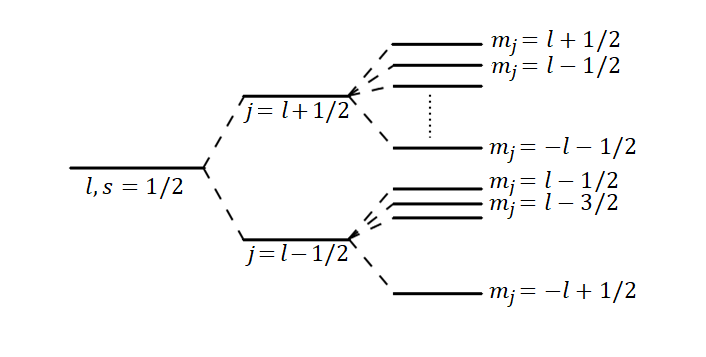
\includegraphics[width=10cm]{immagini/cap_24/fig24_1.png}
\end{center}

La separazione dei livelli indotta dal campo magnetico è nota come \textbf{effetto Zeeman}. \\
Talvolta si parla anche di effetto Zeeman \textbf{anomalo}. Questa denominazione impropria è dovuta storicamente al fatto che, ci si aspettava una separazione dei livelli determinata da $\Delta E_B=\mu_BBm$ in luogo della (\ref{eq:cap24_6}).

\section{Effetto Paschen-Back}
In \textbf{campi magnetici intensi}, in cui $\mu_B B$ è paragonabile agli intervalli della struttura fine o è addirittura più grande, la separazione dei livelli non segue quella prevista dalla formula ($\ref{eq:cap24_6}$). Questo fenomeno è detto \textbf{effetto Paschen-Back}. \\
Il calcolo dell'energia di separazione è assai semplice nel caso in cui la \textbf{separazione dei livelli è grande rispetto agli intervalli della struttura fine}, ma sempre piccola, s'intende, rispetto alle distanze dei livelli in assenza di campo esterno. \\
In queste caso è possibile trascurare, in prima approssimazione, l'accoppiamento spin-orbita e considerare $ H_0+H_B $ come hamiltoniana impterturbata. Questa hamiltoniana commuta con gli operatori \textbf{$\boldsymbol{L_z}$ ed $\boldsymbol{S_z}$}, proiezioni del momento angolare orbitale e dello spin nella direzione individuata dal campo esterno, che rappresentano pertanto \textbf{due buoni numeri quantici}. \\
Lo spostamento dei livelli allora può essere facilmente calcolato: 
\begin{eqnarray}
\Delta E_B & = &\bra{\phi_{lm_lm_s}} H_B \ket{\phi_{lm_lm_s}}=\nonumber  \\
& =& \frac{eB}{2mc}\bra{\phi_{lm_lm_s}} \left( L_z+2S_z  \right)\ket{\phi_{lm_lm_s}} ,
\end{eqnarray}
ossia 
\begin{equation}
\Delta E_B = \mu_B B \left( m_l+2m_s\right) .
\end{equation}
La degenerazione dei livelli che si aveva come l'hamiltonana $H_0$ è ora ridotta dal campo magnetico agli stati che hanno lo stesso valore di ($m_l+2m_s$). \\
\textbf{La struttura fine si sovrappone alla separazione nel campo magnetico}. Essa viene determinata dal valore medio dell'operatore $H_{LS}$ rispetto agli stati con $m_l$ ed $m_s$ determinati:
\begin{eqnarray}
\Delta E_{LS} & =& \bra{\phi_{lm_lm_s}} H_{LS} \ket{\phi_{lm_lm_s}}= \nonumber \\
& = &\frac{1}{2mc^2} \langle \frac{1}{r} \ \frac{dV_c}{dr}   \rangle \bra{lm_Lm_S} \vec{L} \cdot \vec{S} \ket{lm_Lm_S} .
\end{eqnarray}
Utilizzando l'identità:
\begin{eqnarray}
\vec{L} \cdot \vec{S} & = & L_xS_x+L_yS_y+L_zS_z= \nonumber  \\
& = & \frac{1}{4} \left( L_{+}+L_{-} \right)  \left( S_{+}+S_{-}\right)-\frac{1}{4} \left( L_{+}-L_{-} \right) \left( S_{+}-S_{-} \right)+L_zS_z =  \nonumber \\
& = &\frac{1}{2} \left( L_{+}S_{-}+L_{-}S_{+} \right)+ L_zS_z ,
\end{eqnarray}
otteniamo
\begin{equation}
\Delta E_{LS}= \frac{\hbar^2}{2mc^2} \langle \frac{1}{r} \ \frac{dV_c}{dr}   \rangle m_lm_s .
\end{equation}
\end{document}